\section{Proposed Model}
\label{sec:proposed-model}

\subsection{Dataset}
\label{subsec:dataset}

We use the FLAME dataset \cite{FLAME_Dataset}, which contains drone-captured images
of wildfires in northern Arizona.
For this project, we use:
\begin{itemize}
    \item 39,375 images for training/validation
    \item 8,617 images for testing
\end{itemize}

\subsection{Model Architecture}
\label{subsec:model-architecture}

We propose an ensemble of three CNNs (Xception, DenseNet, ResNet) fine-tuned on FLAME,
then distilled into a lightweight MobileNetV3. We will also consider pruning to reduce
model size and speed up inference.

\begin{figure}[h]
    \centering
    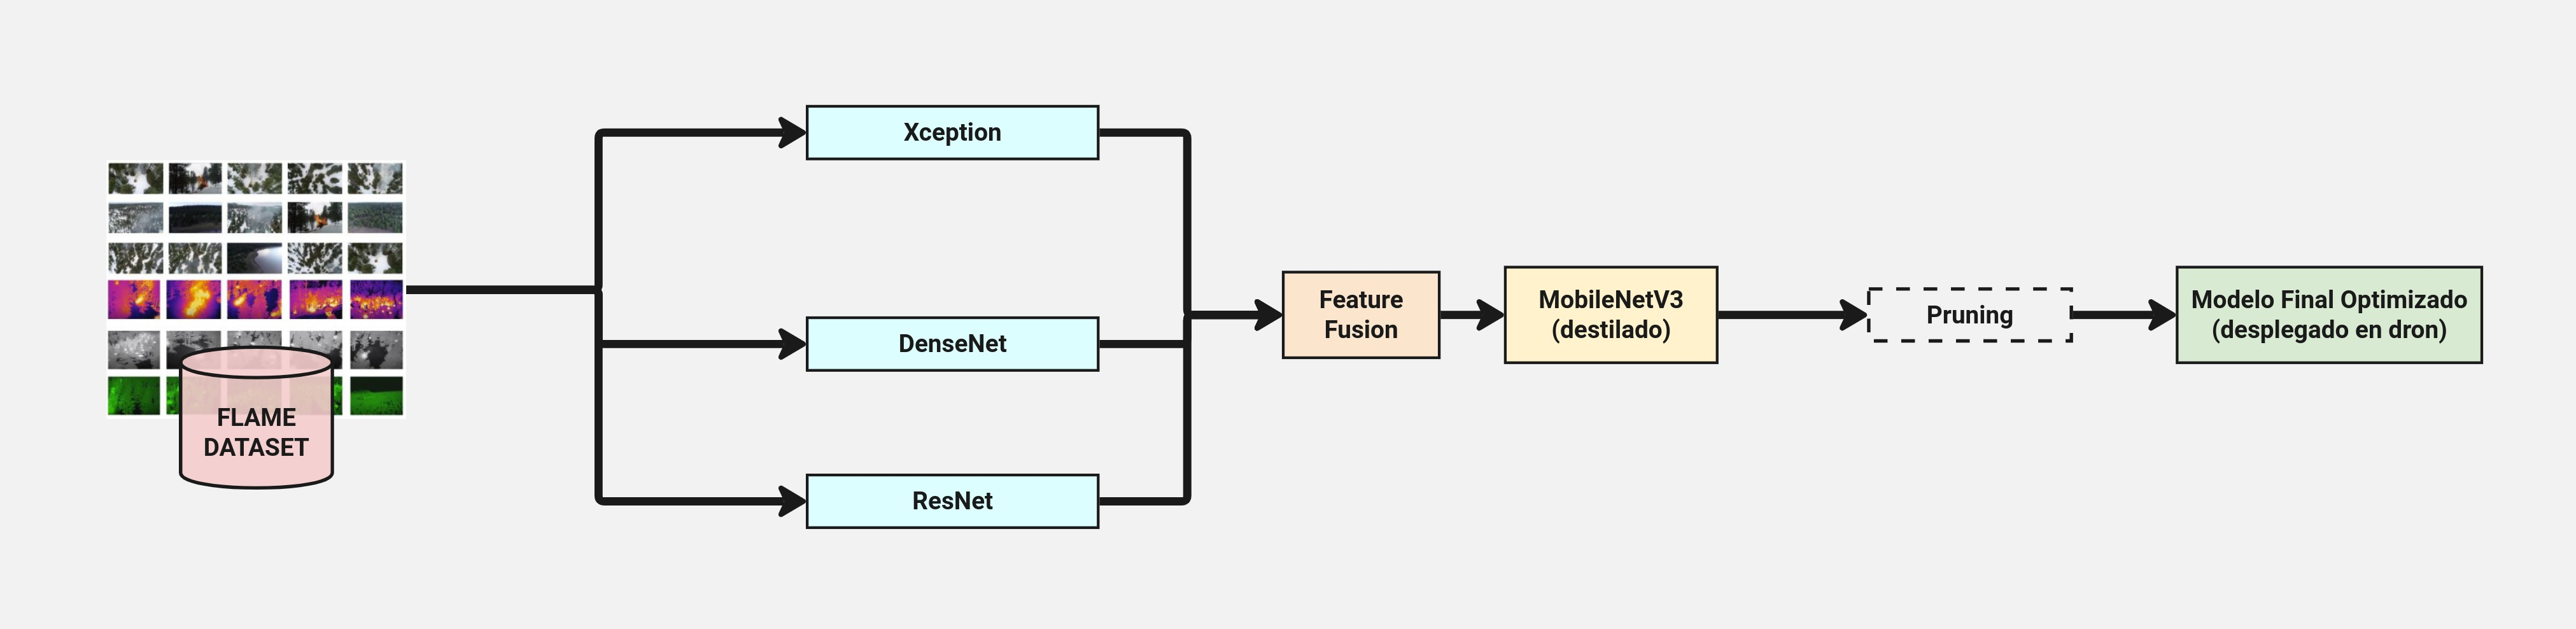
\includegraphics[width=0.9\textwidth]{images/model}
    \caption{Model Diagram}
    \label{fig:model}
\end{figure}

\subsubsection{Training Each Model}
Each CNN is individually trained for binary fire classification using cross-entropy     as the loss function.
Early stopping is used to avoid overfitting.

\subsubsection{Ensemble Fusion}
We explore two strategies:
\begin{enumerate}
    \item \textbf{Final Output Fusion:} Combine each model’s predicted probability by averaging or weighting.
    \item \textbf{Intermediate Feature Fusion:} Extract feature vectors from intermediate layers and train an additional classifier on the fused representations.
\end{enumerate}

\subsubsection{Knowledge Distillation}
Since the ensemble might be too large, we apply knowledge distillation into a MobileNetV3 student model.
This preserves essential knowledge for resource-limited deployment.

\subsection{Justification}
\label{subsec:justification}

\begin{itemize}
    \item \textbf{Xception:} Depthwise separable convolutions for efficient learning.
    \item \textbf{DenseNet:} Dense connectivity improves feature reuse.
    \item \textbf{ResNet:} Residual connections ease training of deep architectures.
    \item \textbf{Distillation into MobileNetV3:} Light and efficient, suitable for real-time drone systems.
\end{itemize}

\subsection{Pipeline}
\label{subsec:pipeline}

\begin{enumerate}
    \item \textbf{Train DenseNet}
    \item \textbf{Train ResNet}
    \item \textbf{Train Xception}
    \item \textbf{Ensemble the models}
    \item \textbf{Distill the ensemble into MobileNetV3}
\end{enumerate}
A shell script (\texttt{scripts/run\_pipeline.sh}) orchestrates these steps.




